\chapter{Setting things up}
\section{Installing Python and Jupyter Notebook}
Please follow https://docs.anaconda.com/anaconda/install/index.html

\noindent I might write my own guide in the future.
\section{The Command Line}
In the past, computers didn't have graphical user interface (GUI, pronounced "gooey"). Instead, everyone interacted with the computer using text commands in what we call a command-line interface (CLI). DOS and MS-DOS are perhaps the most well known command line interface operating system. Some Linux distribution still lack GUI and operated text based.
\begin{figure}[ht]
	\centering
	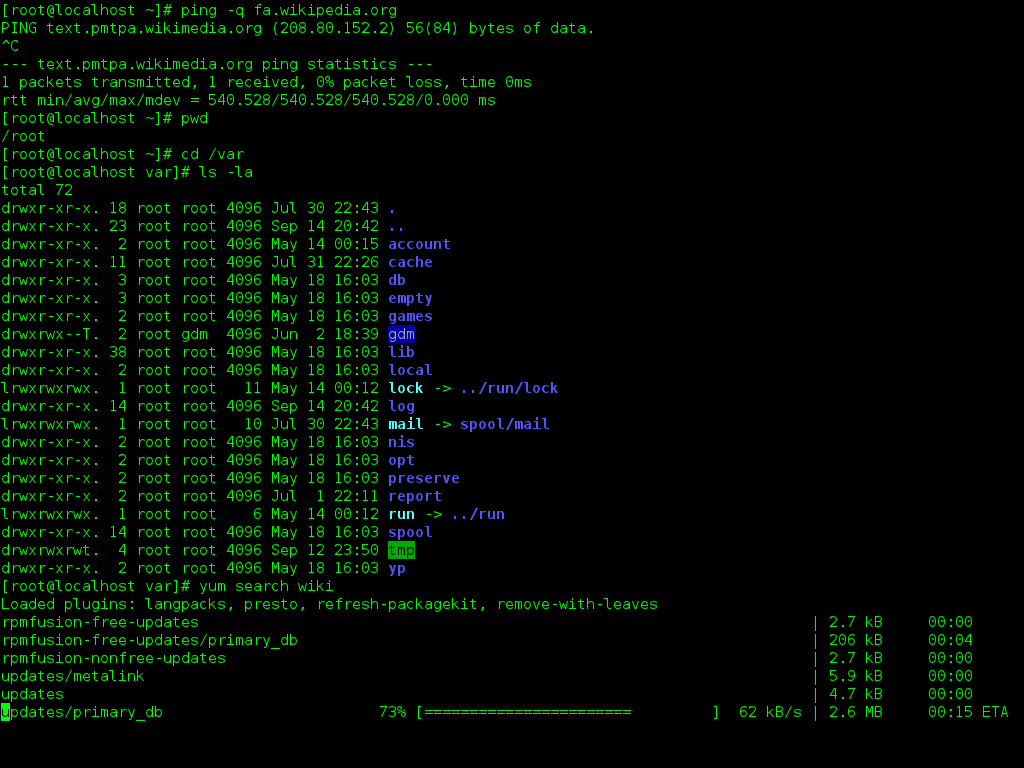
\includegraphics[width=0.5\linewidth]{Assets/Images/Linux_command-line._Bash._GNOME_Terminal._screenshot}
	\caption{Linux Command Line.}
	\label{fig:linuxcommand-line}
\end{figure}

\noindent A shell (or terminal) is a type of command-line program that contains a simple, text-based user interface, enabling us to access all of an operating system's services. It is, put simply, a program that accepts text as an input and translates that text into the appropriate functions you want your computer to run.

\noindent It might look cumbersome but everything we can do with GUI can also be done with command line, often faster. It just doesn't look pretty.
\subsection{How to Access Terminal}
It is extremely simple for Linux users, you can just type "terminal" on your program search.

\noindent Windows users have several options:
\begin{itemize}
	\item \textbf{Windows Command Prompt}: Also known as cmd. A legacy DOS-based shell.
	\item \textbf{Windows PowerShell}: The official Windows-native shell and scripting language, intended to replace the antiquated Command Prompt. 
\end{itemize}

\noindent Alternatively, there are several others third party programs available, such as GitBash and the built in cmd-prompt and PowerShell in Anaconda.

\subsection{Shell Commands}

Here is a list of commonly used shell commands.

\begin{tabular}{|c|c|}
	\hline
	Commands &  \\
	\hline
	ls & list directory \\
	\hline
	cd & change directory \\
	\hline
	cat & read, create, concatenate files \\
	\hline
	mv & move or rename directory \\
	\hline
	echo & print text to terminal window \\
	\hline
	touch & create files \\
	\hline
	mkdir & make directory \\
	\hline
	man & print manual or get help \\
	\hline
	pwd & print working directory \\
	\hline
	rmdir & remove directory \\
	\hline
	cp & copy data or file \\
	\hline
	head & read the start of file \\
	\hline
	tail & read the end of file \\
	\hline
	exit & exit out of a directory \\
	\hline
	kill & terminate a process \\
	\hline
\end{tabular}
\subsection{Navigating with Terminal}
\subsection{Shell Demonstrations}
image intensive
\section{GIT}
ALWAYS DOUBLE CHECK BEFORE MERGE. Reverting a merge can be a real pain.